\documentclass[12pt, a4papre]{article}
\usepackage[catalan]{babel}
\usepackage[unicode]{hyperref}
\usepackage{amsmath}
\usepackage{amssymb}
\usepackage{amsthm}
\usepackage{xifthen}
\usepackage{listings}
\usepackage{float}
\usepackage{graphicx}

\newcommand{\norm}[1]{\lvert #1 \rvert}
\graphicspath{ {./Images/Practica1/} }
\setlength\parindent{24pt}

\hypersetup{
    colorlinks = true,
    linkcolor = blue
}

\author{Elias Ismael Estévez\\Daniel Vilardell}
\title{Memoria practica 1 ICOM}
\date{}

\begin{document}
	\maketitle
	
	\textbf{Comentari:} Fent la practica ens en vam adonar que el resultat del exercici 1.2 del previ era erroni, ja que les simulacions no donaven com haviem esperat, així que aqui esta repetit ben fet.
	
	Tenim que 
	\[
		P_L = \frac{|V_g|^2}{2(R_L + R_g)}R_L = 10^{-4} W = 0.1 mW \implies 
	\]
	\[
		\implies P_L(dBm) = 10log(0.1) = -10 dBm
	\]
	\newpage
	\textbf{Qüestió 1 i 2:}
	
	Podem veure clarament que la potencia del harmonic principal es la esperada, es a dir, -10 dBm. No podem arribar a visualitzar els harmonics secundaris del tot ja que el span es massa petit i el harmonic principal esta centrat, tot i això encara es veu el començament del segon harmonic a la dreta.
	
	\begin{figure}[H]
		\begin{center}
		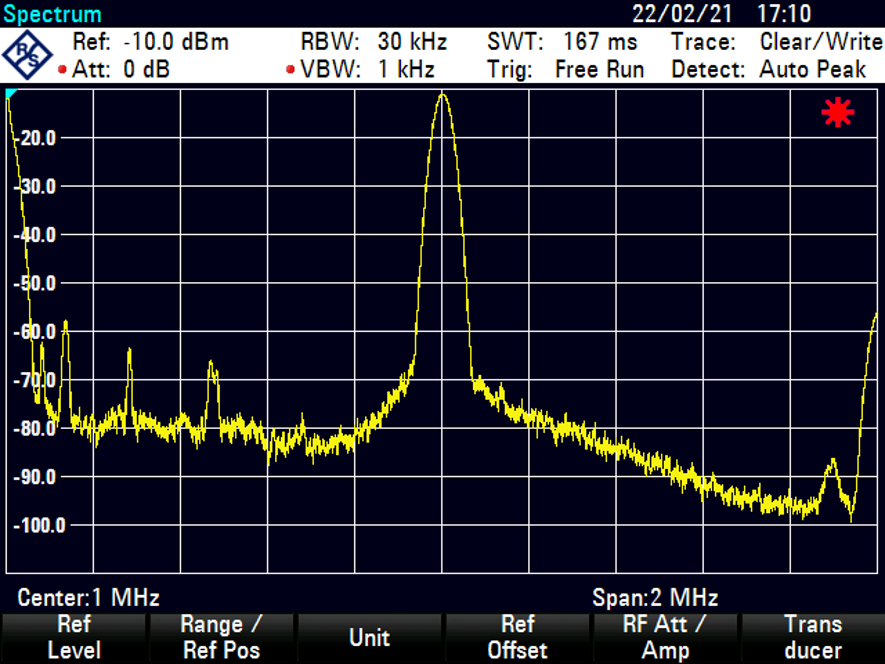
\includegraphics[width=80mm]{2.png}
		\caption{Captura del analitzador d'espectres}
		\end{center}
	\end{figure}
	
	
	
	\textbf{Qüestió 3:}
	
	Podem arribar a mesurar l'ample de banda del senyal a partir dels Markers, que tenim a $54.2kHz$ de separació i a $3.2dB$ de diferencia de potencia. Per tant l'ample de banda es de aproximadament $BW = 2\cdot 50 = 100kHz$.
	
	\begin{figure}[H]
		\begin{center}
		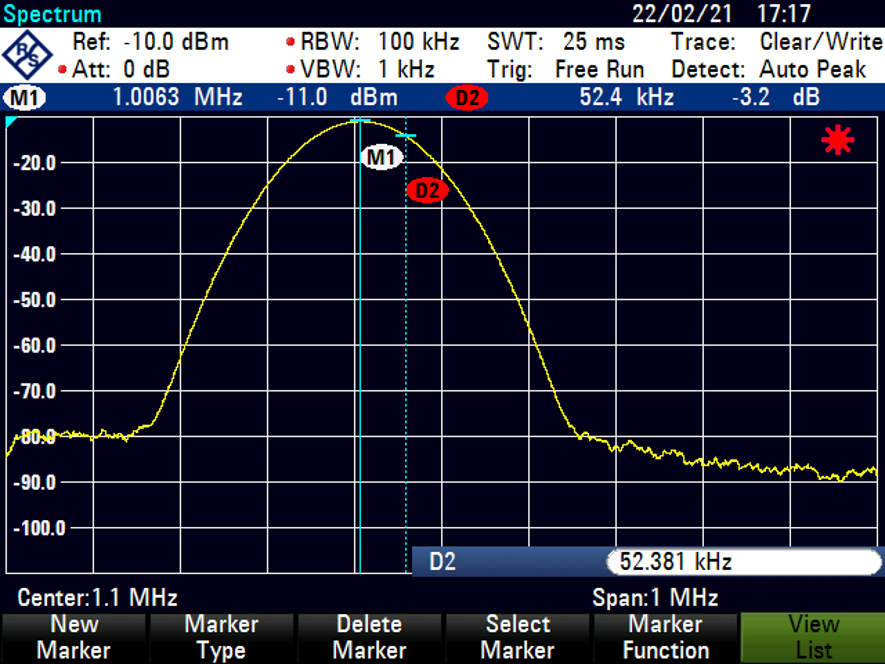
\includegraphics[width=110mm]{3.png}
		\caption{Captura del analitzador d'espectres}
		\end{center}
	\end{figure}
	
	Finalment, provant amb altres frequencies veiem que els harmonics secundaris s'incrementen fins a solapar amb el principal i modificarlo.
	
	\textbf{Qüestió 4:} Quan s'agafa 0 span el senyal es queda a un mateix lloc i no es mou, cosa que fa que el resultat sigui una sinusoide de frequencia igual a la frequencia del filtre menys la del center frequency. Si agafem el envolvent d'aquesta senyal ens donara la potencia de la senyal a la frequencia seleccionada com a valor de continua. Veiem que si posem la center frequency al pic obtenim un valor de -10dB, com haviem obtingut al pic del senyal mostrat amb un span diferent de 0. Si movem el center frequency com podem veure a la segona imatge el valor de potencia disminueix.
	
	\begin{figure}[H]
		\begin{center}
		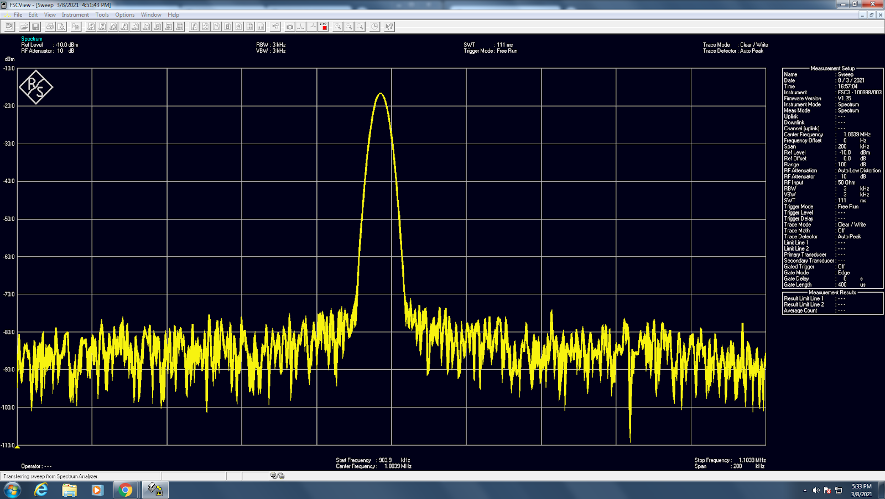
\includegraphics[width=80mm]{4_3.png}
		\caption{Captura del analitzador d'espectres abans de posar zero span}
		\end{center}
	\end{figure}
	
	\begin{figure}[H]
		\begin{center}
		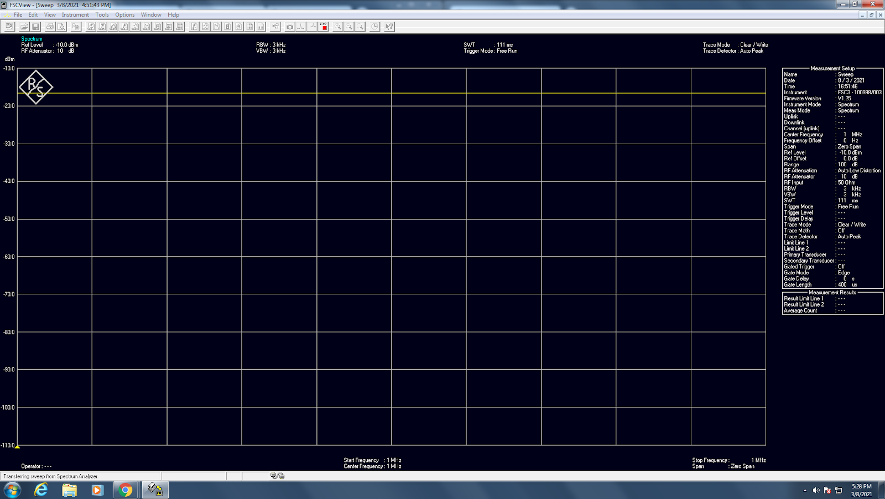
\includegraphics[width=80mm]{4_1.png}
		\caption{Captura del analitzador d'espectres amb center frequency = 1MHz}
		\end{center}
	\end{figure}
	
	\begin{figure}[H]
		\begin{center}
		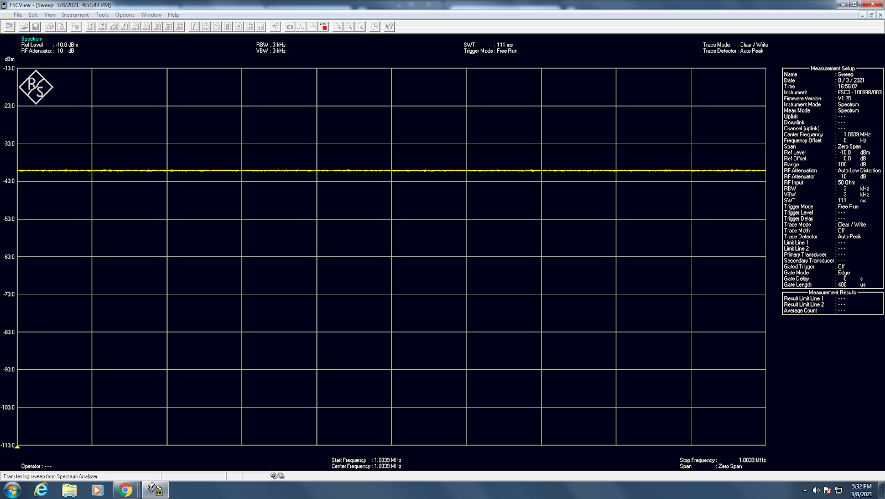
\includegraphics[width=80mm]{4_2.png}
		\caption{Captura amb center frequency = 1.0039MHz}
		\end{center}
	\end{figure}
	
	\textbf{Qüestió 5:} 
	
	\begin{figure}[H]
		\begin{center}
		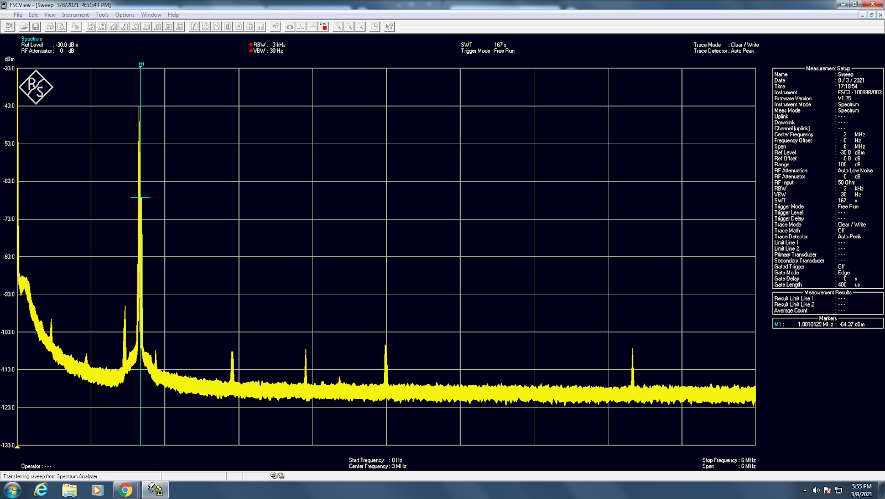
\includegraphics[width=110mm]{5.png}
		\caption{Captura on es veuen els primers 4 harmonics}
		\end{center}
	\end{figure}
	
	Els metodes usats amb el fi de reduir el soroll son reduir el VBW, cosa que hem arribat a fer fins a 30Hz, també posar el mode d'atenuació a low noice i finalment reduir el RBW. El que ens donava una senyal mes nitida però era el VBW, tot i que incrementava molt el temps de escombratge del analitzador d'espectres.
	
\end{document}










